\documentclass[]{article}
%Busca la linea que pone /tableofcontents y empieza a escribir debajo de cada sección.
%Te explico para qué es cada cosa que sea medio relevante:
\usepackage{amsmath}
\usepackage{amssymb}
\usepackage{verbatim} %con verbatim escribes bloques de texto con letra mono.
\usepackage{graphicx} %para insertar imagenes, cuando meta yo una usa el codigo de ejemplo
\usepackage{listings}
\usepackage{fullpage}
\usepackage{color}
\usepackage{fancyvrb}
\usepackage[spanish]{babel}
\usepackage[utf8]{inputenc} %Para usar acentos directamente en latex
\usepackage{hyperref} %Para que el indice tenga hiperenlaces y si quieres poner los tuyos
\hypersetup{%
	pdfborder = {0 0 0}
}

\definecolor{mygreen}{rgb}{0,0.6,0}
\definecolor{mygray}{rgb}{0.5,0.5,0.5}
\definecolor{mymauve}{rgb}{0.58,0,0.82}

%Para insertar código: crea un recuadro con texto mono y lineas enumeradas. Puedes referenciar un fichero y no copiar y pegar aquí.
\lstset{ %
	backgroundcolor=\color{white},   % choose the background color; you must add \usepackage{color} or \usepackage{xcolor}
	basicstyle=\footnotesize,        % the size of the fonts that are used for the code
	breakatwhitespace=false,         % sets if automatic breaks should only happen at whitespace
	breaklines=true,                 % sets automatic line breaking
	captionpos=b,                    % sets the caption-position to bottom
	commentstyle=\color{mygreen},    % comment style
	 keywordstyle=\color{blue}, % keyword color
	 stringstyle=\color{red} % string color
	frame=single,                    % adds a frame around the code
	keepspaces=true,                 % keeps spaces in text, useful for keeping indentation of code (possibly needs columns=flexible)
	numbers=left,                    % where to put the line-numbers; possible values are (none, left, right)
	numbersep=5pt,                   % how far the line-numbers are from the code
	numberstyle=\tiny\color{mygray}, % the style that is used for the line-numbers
	rulecolor=\color{black},         % if not set, the frame-color may be changed on line-breaks within not-black text (e.g. comments (green here))
	showspaces=false,                % show spaces everywhere adding particular underscores; it overrides 'showstringspaces'
	showstringspaces=false,          % underline spaces within strings only
	showtabs=false,                  % show tabs within strings adding particular underscores
	stepnumber=1,                    % the step between two line-numbers. If it's 1, each line will be numbered
	stringstyle=\color{mymauve},     % string literal style
	tabsize=4,                       
	title=\lstname                   % show the filename of files included with \lstinputlisting; also try caption instead of title
}



\title{Laboratorio de Programación de Sistemas Embebidos en Red}
\author{José Luis Cánovas Sánchez\\Ezequiel Santamaría Navarro}

\begin{document}

\maketitle


\begin{abstract}
En nuestra práctica final del laboratorio hemos integrado todos los sensores estudiados en la primera parte con un servidor web integrado en una raspberry pi. Por eso dividimos la memoria en describir los sensores y arduino (la primera parte de las prácticas), y la segunda en el código final que comunica la raspberry pi y arduino (la segunda parte de trabajo propio).
\end{abstract}

\tableofcontents

\clearpage

\section{Práctica 1. Introducción a Arduino. Descripción del hardware}
Para poder utilizar directamente un cable entre la Raspberry Pi y Arduino, sin necesidad de un divisor de tensión para pasar de 5v de Arduino UNO a 3.3v de la Raspberry Pi, usamos la versión de Arduino DUE, que usa en sus pines 3.3v. Esto sólo afectará a la comunicación Arduino-Raspberry y al Led, porque son los únicos que se conectan directamente a un pin de Arduino, porque el resto de sensores los conectamos al pin de 5v que ofrece Arduino DUE, y la entrada de datos se realiza por los puertos analógicos.

Vamos a describir brevemente en cada apartado cómo integramos cada sensor con el Arduino. En la  \autoref{fig:squemadibujo} se ve el sistema global donde se puede comprobar cada esquema individual.

\begin{figure}[h!]
	\centering
	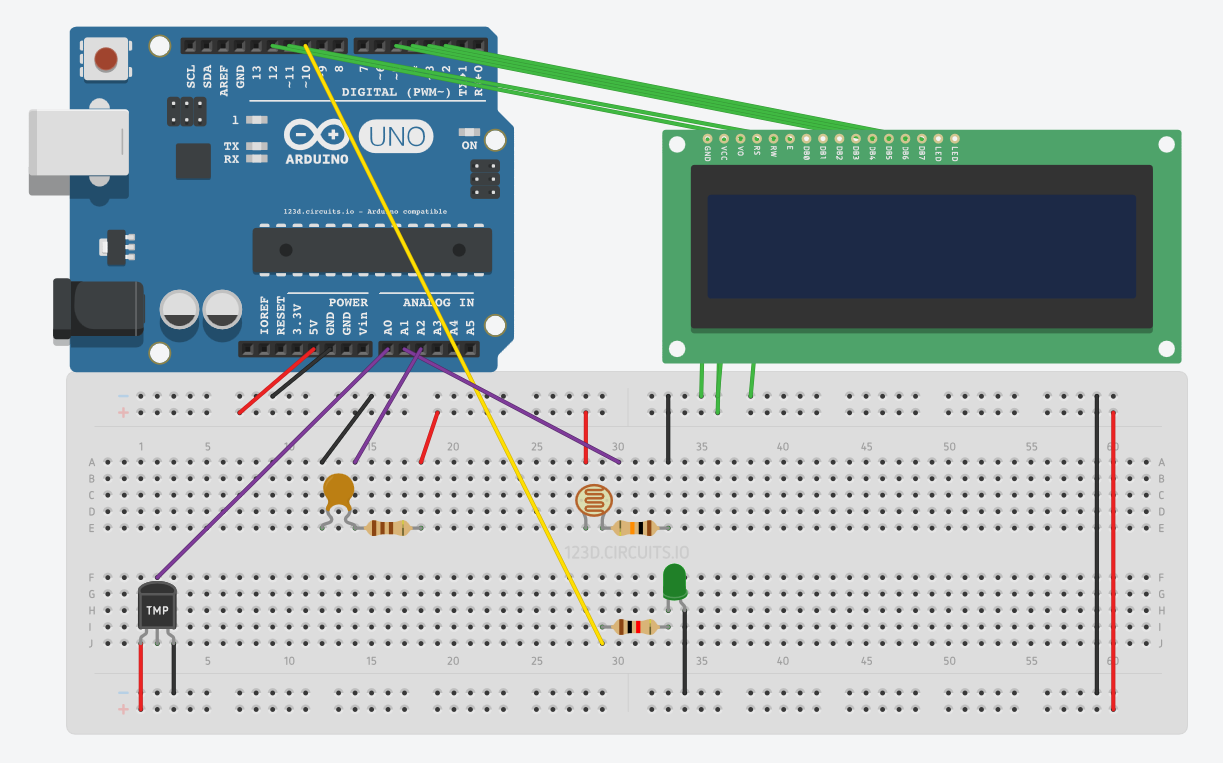
\includegraphics[width=1\linewidth]{images/squemaDibujo.PNG}
	\caption{Esquema global}
	\label{fig:squemadibujo}
\end{figure}


\begin{figure}[h!]
	\centering
	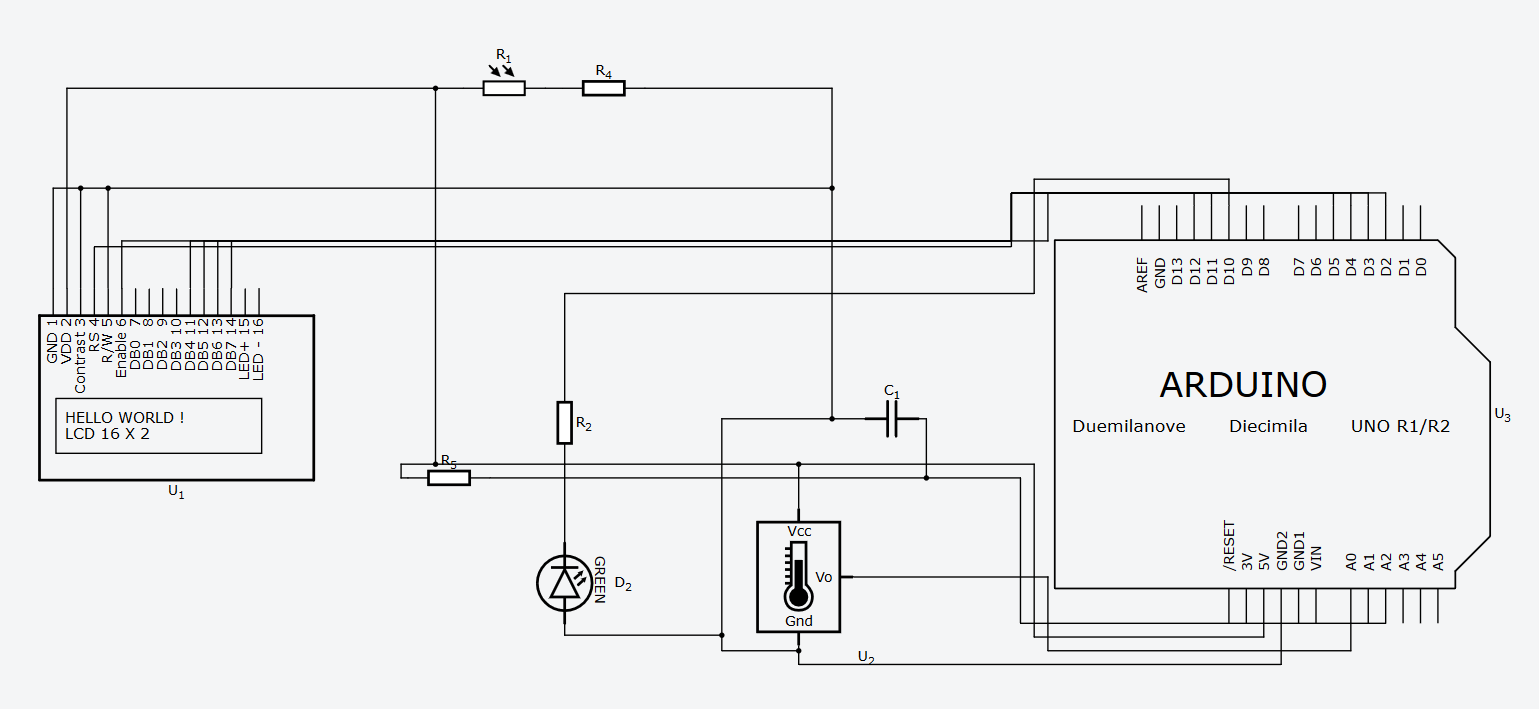
\includegraphics[width=0.6\linewidth]{images/squema.PNG}
	\caption{Esquema global}
	\label{fig:squema}
\end{figure}


\subsection{Led}

\subsection{Sensor de luz}

\subsection{NTC}

\subsection{LDR}

\subsection{LCD}

\subsection{Generador señal tipo GPS}

\lstinputlisting[language=C++,frame=single]{senialGPS.ino}


\section{Práctica 2. Montaje de un servidor web de monitorización. Descripción del software}

En la segunda parte de la práctica hemos puesto como objetivo desarrollar algo en el ámbito de internet de las cosas. Básicamente nuestro reto ha sido poner en internet (en nuestro caso usando HTTP y servicios Web) los distintos sensores y el monitor LCD utilizados en la práctica anterior.

Para ello nos hemos servido de un Arduino Due (ya que el voltaje de sus pines es compatible con la Raspberry Pi), de una Raspberry Pi y de un router Wifi que hace de punto de acceso entre la Raspberry Pi e internet.

\subsection{Montaje de red}
%TODO: Poner un esquema

La Raspberry Pi, por su gran capacidad de cómputo, hace de centro de datos. Recibe información del Arduino Due a través de el puerto serie, y lo pone en internet a través de un puerto Ethernet. 

\subsection{Protocolo serie}
%TODO: Completar con la especificación.

El protocolo serie es muy simple, y se basa en transmitir unas tramas con la siguiente información (en ese orden):

\begin{itemize}
	\item 4 bytes que codifican en ASCII hexadcimal el tamaño de la trama.
	\item 1 byte que codifica en ASCII el tipo del paquete. Puede ser %TODO
	\item Varios bytes con el payload de la trama, en ASCII. No pueden contener el byte 0.
	\item 1 byte nulo (valor 0) que inidica fin de la trama. Se utiliza para sincronizar en caso de error.
\end{itemize}

\subsection{Código arduino}

Lo primero que hemos hecho ha sido reutilizar parte del código de la primera práctica. En un bucle continuo, leemos los sensores de temperatura y luz y con la información obtenida mandamos frames por el protocolo serie a la Raspberry Pi.

\hfill

Por otro lado, también nos encargamos de leer frames que puedan venir de la Rapsberry Pi. Si llega un frame de tipo 'L', le cambiamos el valor al \textit{analog output} del led, haciendo que ilumine más o menos. O por si llega un frame de tipo 'D', en cuyo caso limpiamos el display y ponemos el nuevo texto en la pantalla.

\subsection{Servicio web}
El servicio web tiene dos partes, un código escrito en python que corre en la Rapsberry PI y otro código escrito en javascript que se ejecuta en un teléfono móvil, o un pc.

\subsubsection{Parte servidor de python}
En esta parte, se espera a que un navegador web estándar haga una petición de tipo GET para obtener el documento index.html. Además, está a la espera de recibir peticiones GET al documento 'luz' o al documento 'tmp'.

\hfill

Cada vez que recibe una petición al documento luz, lee las tramas a través del puerto serie para obtener del Arduino la última lectura del sensor de luz. Después, contesta la petición con el valor del sensor. Lo mismo sucede si se recibe una petición al documento tmp, solo que se devuelve la temperatura.

\hfill

Por otro lado, el servidor de python también está a la espera de las peticiones PUT 'led' y 'display'. En este caso, en vez de devolver un valor leyendo por el puerto serie, lo que hace es escribir en el puerto serie una trama de tipo 'L' (si led) o de tipo 'D' (si display) para alterar el brillo del led o el texto del monitor LCD.

\subsubsection{Parte cliente de javascript}

En el explorador web, se ejecuta continuamente una petición de tipo GET 'luz' y GET 'tmp', para actualizar en tiempo real la oscuridad del fondo (dependiendo del nivel de luz), o el valor de un número dependiendo de la temperatura.

\hfill

También se pone una barra de desplazamiento para modificar el brillo del led, y una barra de texto para cambiar el mensaje del display. Cuando se mueve la barra de desplazamiento se ejecuta un PUT 'led', y cuando se cambia el texto en la barra se ejecuta un PUT 'display', que llegan al servidor web de python.


%TODO: Poner una imagen de ejemplo del sistema. Si no hay, poner un esquema o un dibujo.

\section{Notas adicionales}

\subsection{Aproximación a la temperatura real}
Siguiendo las indicaciones de los fabricantes de los sensores de temperatura hemos llegado a lecturas que no pueden corresponderse con la realidad (porque aparecían disparates), así que hemos tenido que aproximar la temperatura con la experimentación.

%TODO: Exponer las fórmulas

\subsection{Lector de pulsaciones}
%TODO: Hablar del lector de pulsaciones

\section{Código}
\subsection{Código Arduino}

Dos ficheros, uno con el código de los sensores de la primera parte, usando el Arduino UNO, y el segundo el código de Arduino DUE con el protocolo de comunicación y lectura de sensores.


\textit{Código sensores Arduino UNO:}
\lstinputlisting[language=C++,frame=single]{codigoSensoresArduinoUNO.ino}

\textit{Código Arduino DUE:}
\lstinputlisting[language=C++,frame=single]{pser.ino}

\subsection{Código Raspberry Pi}

Dos ficheros, el servidor web escrito en Python, implementando el protocolo de comunicación con Arduino DUE, y el fichero \textit{index.html} de la página web que muestran la información de los sensores o entrada de datos para pantalla y led.

\textit{Código servidor Python:}
\lstinputlisting[language=Python,frame=single]{restserver.py}

\textit{Código página web:}
\lstinputlisting[language=html,frame=single]{index.html}

\end{document}
